%\documentclass[12pt,twoside]{report} % Use esta linha para tese com mais de 100 p{\'a}ginas
\documentclass[12pt]{report} % Use esta linha para tese com at{\'e} 100 p{\'a}ginas

% Definições do IC-Unicamp
\usepackage{ic-tese}

% Definições latex para portugues
\usepackage[utf8]{inputenc}
\usepackage[brazil]{babel}
\usepackage[T1]{fontenc}

% Formatação de URL
\usepackage{url}

% Adição de figuras no documento
\usepackage{graphicx}

% Tabelas longas (mais de uma página)
\usepackage{longtable}
\usepackage{rotating}
\usepackage{array}
\usepackage{multirow}

% Formatação de códigos
\usepackage[algoruled]{algorithm2e}
\usepackage{listingsutf8}
\usepackage{xcolor}
\usepackage{framed}

% Definições matemáticas
\usepackage{amsmath}
\usepackage{amsfonts}
\usepackage{amsthm}

% incluir pdf
\usepackage{pdfpages}

% Hiperlinks
\usepackage[pdftex,colorlinks=true,allcolors=black]{hyperref}

% Definições de hifenização
\hyphenation{a-de-qüa-dos a-li-nha-dos a-li-nha-men-to
  a-li-nha-men-tos a-lign-ments a-tra-vés BAliBASE e-xem-plo
  ge-ne-ra-li-za-da glo-bal-men-te pu-bli-ca-das re-fe-rên-cia
  re-pe-ti-ções se-me-lhan-ça UPGMA vi-zi-nhas}

\newcommand{\aspas}[1]{``#1''}
\newcommand{\estr}[1]{\textsl{\foreignlanguage{american}{#1}}}

\newcommand{\ic}{Instituto de Computação}
\newcommand{\bkp}{\textit{breakpoints}}
\newcommand{\pli}{programação linear inteira}
\newcommand{\PLI}{Programação Linear Inteira}
\newcommand{\pr}{programação por restrições}
\newcommand{\PR}{Programação por Restrições}
\newcommand{\plr}{programação lógica por restrições}
\newcommand{\PLR}{Programação Lógica por Restrições}
\newcommand{\unicamp}{Universidade Estadual de Campinas}

\newtheorem{teo}{Teorema}[chapter]
\newtheorem{defin}{Definição}[chapter]

\begin{document}
  
\thesislanguage{3} % PT-BR

\thetitle{Programação por Restrições aplicada a Problemas de Rearranjo de
    Genomas.}

\thisyear{2012}

\author{Victor de Abreu Iizuka}

\degreesoughtpt{Mestrado} % Doutorado/Mestrado
\degreesought{MSc} % Doutorado/Mestrado

\titlesoughtpt{Mestre}     % Doutor(a)/Mestre
\titlesought{Master}     % Doutor(a)/Mestre

\principaladvisor{Prof. Dr. Zanoni Dias}
\advisortitle{Orientador} % Orientadora

%\coadvisor{Byron Meter (Co-orientador)} % Pode ser omitido.

\firstreader{Prof. Dra. Maria Emília Machado Telles Walter\\Departamento de
  Ciência da Computação -- CIC -- UnB}

\secondreader{Prof. Dr. Guilherme Pimentel Telles\\Instituto de Computação --
  Unicamp}

\thirdreader{Prof. Dr. Nalvo Franco de Almeida Junior
  (Suplente)\\Faculdade de Computação -- UFMS}

\fourthreader{Prof. Dr. João Meidanis (Suplente)\\Instituto de
  Computação -- Unicamp}

\grants{{\rm Suporte financeiro de: Bolsa da CNPq (processo 134380/2009-6)
03/2009--03/2011 } } % Pode ser omitido.

\defencedate{19}{12}{2012} % dia mes ano

%   Se pretende utilizar \copyrighttrue, consulte antes seu orientador ou a CPG!!!
%   Este ponto envolve quest{\~o}es legais complexas e de graves conseq{\"u}{\^e}ncias.
\copyrightfalse % Caso nao queira que apareca a pagina de Copyright.
%    \copyrighttrue % Caso queira que apareca a pagina de Copyright.

%    \finalversiontrue % Caso seja a versao final.
\finalversionfalse % Caso nao seja a versao final ainda.
%
\tablespagetrue % Caso queira que apareca a Lista de Tabelas.
%    \tablespagefalse % Caso nao queira que apareca a Lista de Tabelas.
%
\figurespagetrue % Caso queira que apareca o Lista de Figuras.
%    \figurespagefalse % Caso nao queira que apareca o Lista de Figuras.
%

\beforepreface

\prefacesection{Abstract}
% abstract
The evolutionary process was the main responsible for the
differentiation between living beings and one of contemporary theories
about the way as this process occurs states that, during the course of
evolution, genetic changes occurred, creating different kinds of
living beings. Many of these changes are due to point mutation that
modify the DNA sequence, preventing that information is expressed, or
it is expressed in another way. The sequence comparison is the most
common method to characterize the occurrence of point mutation, and is
one of the most discussed problems in Computational Biology. The
interest in making such comparison is to find the edit
distance~\cite{SetubalMeidanis*1997}. The edit distance is a measure
capable of estimating the evolutionary distance between to sequences,
but lacks the information of which global operations were used to
change one sequence in another. These global operations are called the
Genome Rearrangements, which may be, for example, reversals,
transpositions, fissions and fusions. The distance can be defined for
any rearrangement class as the smallest number of operations required
to change one sequence into another. For example, the reversal
distance is the smallest number of reversals required to change one
sequence into another~\cite{BafnaPevzner*1996} and the transposition
distance is the smallest number of
transpositions~\cite{BafnaPevzner*1998}. This work follows the
research line used by Dias e Dias~\cite{DiasDias*2009} and we
introduce Constraint Logic Programming models for sorting by reversals
and sorting by reversals and transpositions, based on Constraint
Satisfaction Problems theory and Constraint Optimization Problems
theory. We made a comparison between the Constraint Logic Programming
models for sorting by transpositions, described in Dias and
Dias~\cite{DiasDias*2009}, sorting by reversals and sorting by
reversals and transpositions, with the Integer Linear Programming for
the same problems described in Dias and Souza~\cite{DiasSouza*2007}.



\prefacesection{Resumo}
% resumo
O processo evolutivo foi o principal responsável pela diferenciação
entre os seres vivos e uma das teorias contemporâneas acerca do modo
como ocorre esse processo afirma que, durante o curso da evolução,
mudanças genéticas aconteceram, criando diferentes espécies de seres
vivos. Muitas dessas mudanças são devido a mutações pontuais que
alteram a cadeia de DNA, impedindo que a informação seja expressa, ou
que seja expressa de um modo diferente. A comparação de sequência é o
método mais usual de se caracterizar a ocorrência de mutações
pontuais, sendo um dos problemas mais abordados em Biologia
Computacional. O interesse em fazer tal comparação é encontrar a
distância de edição~\cite{SetubalMeidanis*1997}. A distância de edição
é uma medida capaz de estimar a distância evolutiva entre duas
cadeias, mas não possui a informação de quais operações globais foram
utilizadas para a transformação de uma sequência em outra. Estas
operações globais são os chamados Rearranjos de Genomas, que podem
ser, por exemplo, reversões, transposições, fissões e fusões. Um
conceito de distância pode ser definido para qualquer classe de
rearranjo como sendo o menor número de operações pertencentes a essa
classe que são necessários para transformar um genoma em outro. Por
exemplo, chama-se a distância de reversão o menor número de reversões
necessárias para transformar um genoma em
outro~\cite{BafnaPevzner*1996} e a distância de transposição é o menor
número de transposições~\cite{BafnaPevzner*1998}. Este trabalho segue
a linha de pesquisa utilizada por Dias e Dias~\cite{DiasDias*2009} e
nós apresentaremos modelos de Programação por Restrições para
ordenação por reversões e ordenação por reversões e transposições,
baseados na teoria do Problema de Satisfação de Restrições e na teoria
do Problema de Otimização com Restrições. Nós fizemos comparações com
os modelos de Programação por Restrições para ordenação por
transposições, descrito por Dias e Dias~\cite{DiasDias*2009},
ordenação por reversões e ordenação por reversões e transposições com
os modelos de Programação Linear Inteira para os mesmos problemas
descritos em Dias e Souza~\cite{DiasSouza*2007}.


\prefacesection{Agradecimentos}
Gostaria de agradecer aos meus pais que fizeram tudo de possível para
eu conseguir chegar até aqui, dando apoio e aquele ``puxão de orelha''
sempre quando precisou, ao meu irmão que sempre me ajuda quando
preciso e a todos os familiares que me apoiaram durante esse período.

Agradeço também ao professor Zanoni por ter auxiliado em todo o
momento em que estive com dúvidas e pela paciência dispensada durante
a orientação.

Finalmente, agradeço a todos os meus amigos, porque sem eles
certamente não seria possível continuar esse trabalho.


\afterpreface % Gera: Conteudo, Lista de Tabelas, Lista de Figuras.

\chapter{Introdução}
\label{cap:intro}
% introducao
O processo evolutivo foi o principal responsável pela diferenciação
entre os seres vivos e uma das teorias contemporâneas acerca do modo
como ocorre esse processo afirma que, durante o curso da evolução,
mudanças genéticas aconteceram criando diferentes espécies de seres
vivos.

Muitas dessas mudanças são devido a mutações pontuais que alteram a
cadeia de DNA, impedindo que a informação seja expressa, ou que seja
expressa de um modo diferente. Tais alterações debilitam, na maioria
dos casos, o organismo portador ou proporcionam vantagens no processo
de seleção natural.

A comparação de sequência é o método mais usual de se caracterizar a
ocorrência de mutações pontuais, sendo um dos problemas mais abordados
em Biologia Computacional. O interesse em fazer tal comparação é
encontrar a distância de edição~\cite{SetubalMeidanis*1997}, que é o
número mínimo de operações de inserções, remoções e substituições
necessárias que transformam uma sequência em outra.

A distância de edição é uma medida capaz de estimar a distância
evolutiva entre duas cadeias, mas não possui a informação de quais
operações globais foram utilizadas para a transformação de uma
sequência em outra. Estas operações globais são os chamados
Rearranjos de Genomas, que podem ser, por exemplo, reversões,
transposições, fissões e fusões.

Um conceito de distância pode ser definido para qualquer classe de
rearranjo como sendo o menor número de operações pertencentes a essa
classe que são necessários para transformar um genoma em outro. Por
exemplo, chama-se a distância de reversão o menor número de reversões
necessárias para transformar um genoma em
outro~\cite{BafnaPevzner*1996} e a distância de transposição é o menor
número de transposições~\cite{BafnaPevzner*1998}.

Estudos mostram que os rearranjos de genomas são mais apropriados que
mutações pontuais quando se deseja comparar os genoma de duas
espécies~\cite{PalmerHerbon*1988}. Nesse contexto, a distância
evolutiva entre dois genomas pode ser estimada pelo conceito de
distância para uma classe de rearranjo definido no parágrafo anterior.

Neste trabalho trataremos os casos em que os eventos de transposição e
reversão ocorrem de forma isolada e os casos quando os dois eventos
ocorrem ao mesmo tempo.

% transposição
O evento de transposição ocorre quando dois blocos adjacentes no
genoma trocam de posição. O problema da distância de transposição é
encontrar o número mínimo de transposições necessárias que transforma
um genoma em outro. Este problema pertence à classe dos problemas
NP-Difíceis e a prova foi apresentada por Bulteau, Fertin e
Rusu~\cite{BulteauFertinRusu*2010}. O melhor algoritmo de aproximação
conhecido possui razão de $1.375$ apresentado por Elias e
Hartman~\cite{EliasHartman*2006}.

% reversão
O evento de reversão ocorre quando um bloco do genoma é invertido. O
problema da distância de reversão é encontrar o número mínimo de
reversões necessárias que transforma um genoma em outro. Neste
problema é importante saber se a orientação dos genes é conhecida,
pois existem algoritmos polinomiais para este caso. Entretanto, se a
orientação dos genes não é conhecida o problema da distância de
reversão pertence à classe de problemas NP-Difíceis, com a prova
apresentada por Caprara~\cite{Caprara*1997}, e o melhor algoritmo de
aproximação conhecido possui razão de $1.375$ apresentado por Berman,
Hannenhalli e Karpinski~\cite{BermanHannenhalliKarpinski*2002}.

% reversão+transposição
Na natureza um genoma não sofre apenas eventos de reversão ou de
transposição, ele está exposto a diversos eventos diferentes. Para
esta situação, iremos estudar o caso onde os eventos de reversão e
transposição ocorrem simultaneamente sobre um genoma. Os trabalhos de
Walter, Dias e
Meidanis~\cite{MeidanisWalterDias*2002,WalterDiasMeidanis*1998} e Lin
e Xue~\cite{LinXue*1999} estudaram o problema de encontrar o número
mínimo de reversões e transposições necessárias para transformar um
genoma em outro.

O trabalho desenvolvido nesta dissertação segue a linha de pesquisa
utilizada por Dias e Dias~\cite{DiasDias*2009} e nós apresentaremos
modelos de Programação por Restrições (CP\footnote{Do
inglês \estr{Constraint Programming}.}) para ordenação por reversões e
ordenação por reversões e transposições, baseados na teoria do
Problema de Satisfação de Restrições (CSP\footnote{Do
inglês \estr{Constraint Satisfaction Problems}.}) e na teoria do
Problema de Otimização com Restrições (COP\footnote{Do
inglês \estr{Constraint Optimization Problems}.}). Nós fizemos
comparações com os modelos de Programação por Restrições para
ordenação por transposições, descrito por Dias e
Dias~\cite{DiasDias*2009}, ordenação por reversões e ordenação por
reversões e transposições com os modelos de Programação Linear Inteira
(ILP\footnote{Do inglês \estr{Integer Linear Programming}.}) para os
mesmos problemas descritos em Dias e Souza~\cite{DiasSouza*2007}.

O texto da dissertação está dividido da seguinte maneira. O
Capítulo \ref{cap:basic} apresenta uma série de conceitos básicos
necessários para o entendimento deste trabalho. O
Capítulo \ref{cap:model} descreve os modelos usados neste trabalho. O
Capítulo \ref{cap:resul} traz a análise dos resultados obtidos durante
o trabalho. O Capítulo \ref{cap:concl} apresenta as conclusões da
dissertação.


\chapter{Conceitos Básicos}
\label{cap:basic}
% conceitos basicos
% 
% Arrumar este capítulo para conter a descrição de como se calcula os
% limitantes para cada operação
%
Neste capítulo faremos uma apresentação dos conceitos básicos
necessários para o entendimento e desenvolvimento deste trabalho. Na
seção \ref{sec:defin} mostraremos as definições usadas no decorrer
deste trabalho. As seções \ref{sec:rev}, \ref{sec:trans}
e \ref{sec:rev_trans} descrevem, respectivamente, os problemas de
ordenação por reversões, ordenação por transposições e ordenação por
reversões e transposições.

\section{Definições}
\label{sec:defin}
Para todos os problemas usamos as seguintes definições.

\textit{Permutação.} 
Para fins computacionais, um genoma é representado por uma $n$-tupla
de genes, e quando não há genes repetidos essa $n$-tupla é chamada de
permutação. Uma permutação é representada como $\pi =
(~\pi_{1}~\pi_{2}~\ldots~\pi_{n}~)$, para $\pi_{i} \in \mathbb{N}$, $0
< \pi_{i} \leq n$ e $i \neq j \leftrightarrow \pi_{i} \neq \pi_{j}$. A
permutação identidade é representada como $\iota =
(~1~2~3~\ldots~n~)$. Para a demonstração dos eventos, usaremos como
base a permutação $\pi = (~4~7~3~6~2~5~1~)$.

\textit{Eventos de rearranjo.}
Os eventos de rearranjo tratados neste trabalho são os eventos de
transposição e reversão quando ocorrem isoladamente e quando ocorrem
de forma conjunta. Os eventos são representados por $\rho$ e são
aplicados a $\pi$ de uma maneira específica.

\section{Ordenação por Reversões}
\label{sec:rev}
Um evento de reversão ocorre quando um bloco do genoma é
invertido. Uma reversão $\rho(i, j)$, para $1 \leq i < j \leq n$,
aplicada ao genoma $\pi = (~\pi_{1}~\pi_{2}~\ldots~\pi_{n}~)$ gera a
permutação $\rho\pi =
(\pi_{1}~\ldots~\pi_{i-1}~\pi_{j}~\pi_{j-1}~\ldots~\pi_{i+1}$
$\pi_{i}~ \pi_{j+1}~\ldots~\pi_{n})$, caso a orientação de $\pi$ não é
conhecida (Figura~\ref{fig:rev_nao_orientada}), e $\rho\pi =
(\pi_{1}~\ldots~\pi_{i-1}~-\pi_{j}~-\pi_{j-1}~\ldots~-\pi_{i+1}$
$-\pi_{i}~ \pi_{j+1}~\ldots~\pi_{n})$, caso a orientação de $\pi$ é
conhecida (Figura~\ref{fig:rev_orientada}). 

\begin{figure}
  \centering
  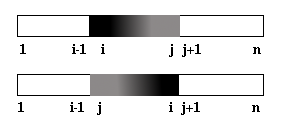
\includegraphics{images/rev_nao_orientada.png} 
  \caption{Reversão em uma permutação não orientada.}
  \label{fig:rev_nao_orientada}
\end{figure}

\begin{figure}
  \centering
  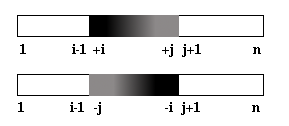
\includegraphics{images/rev_orientada.png}
  \caption{Reversão em uma permutação orientada.}
  \label{fig:rev_orientada}
\end{figure}

A distância de reversão $d_{r}(\pi,\sigma)$ entre duas permutações
$\pi$ e $\sigma$ é o número mínimo $r$ de reversões $\rho_{1}$,
$\rho_{2}$,~$\ldots$~, $\rho_{r}$ tal que
$\pi \rho_{1} \rho_{2}~\ldots~\rho_{r} = \sigma$. Note que a distância
de reversão entre $\pi$ e $\sigma$ é igual à distância de reversão
entre $\sigma^{-1} \pi$ e $\iota$. Então, sem perda de generalidade,
podemos dizer que o problema da distância de reversão é equivalente ao
problema de ordenação por reversões, que é a distância de reversão
entre a permutação $\pi$ e a permutação identidade $\iota$, denotado
por $d_{r}(\pi)$.

Em um estudo inicial sobre este problema, Bafna e
Pevzner~\cite{BafnaPevzner*1996} apresentaram um algoritmo de
aproximação com razão de $1.5$ quando a orientação de genes é
conhecida e $1.75$ caso contrário.

Conhecer a orientação dos genes em um genoma é um fator importante no
problema de reversão, pois existem algoritmos polinomiais para o caso
em que a orientação é conhecida. No caso em que não se conhece a
orientação dos genes o problema de encontrar a distância de reversão
pertence à classe dos problemas NP-Difíceis~\cite{Caprara*1997}.

O primeiro algoritmo polinomial para o problema de reversão com
orientação conhecida foi criado por Hannenhalli e
Pevzner~\cite{HannenhalliPevzner*1995} que fez uso de várias operações
aplicadas a uma estrutura intermediária conhecida como grafo
de \bkp{}. A estratégia usada por Hannenhalli e Pevzner foi
simplificada no trabalho de Bergeron~\cite{Bergeron*2005}. Atualmente
já existe um algoritmo com complexidade
sub-quadrática~\cite{TannierSagot*2004} e, quando apenas a distância é
necessária, um algoritmo linear pode ser
usado~\cite{BaderMoretYan*2001}.

Um resultado importante obtido por Meidanis, Walter e
Dias~\cite{MeidanisWalterDias*2000}, mostrou que toda teoria sobre
reversões desenvolvida para genomas lineares pode ser adaptada
facilmente para genomas circulares, que são comuns em seres inferiores
como vírus e bactérias.

Quando a orientação dos genes não é conhecida existem algoritmos de
aproximação que seguiram a ideia do trabalho de Bafna e Pevzner citado
anteriormente como, por exemplo, o algoritmo implementado por Berman,
Hannenhalli e Karpinski~\cite{BermanHannenhalliKarpinski*2002} com
razão de aproximação de $1.375$.

\subsection{Ferramentas para o Problema de Ordenação por Reversões.}
\label{subsec:toolrev}
O conceito de grafo de \bkp{} foi introduzido no trabalho de Bafna e
Pevzner~\cite{BafnaPevzner*1996}. Inicialmente a permutação $\pi$ é
estendida adicionando o elemento $\pi_{0} = 0$ e $\pi_{n+1} =
n+1$. Dois elementos consecutivos $\pi_{i}$ e $\pi_{i+1}$, $0 \le
i \le n$, são \textit{adjacentes} quando $|\pi_{i} - \pi_{i+1}| = 1$,
e são \estr{breakpoints} caso contrário. Define-se um grafo de arestas
coloridas $G(\pi)$ com $n + 2$ vértices \{0, 1,~$\ldots$~, $n$, $n +
1$\}. Unimos os vértices $i$ e $j$ com uma aresta preta se $(i, j)$
for um \estr{breakpoint}. Unimos os vértices $i$ e $j$ com uma aresta
cinza se $|i - j| = 1$ e $i$, $j$ não são consecutivos em
$\pi$. Denotamos por $b_r(\pi)$ o número de \bkp{} existentes em
$\pi$. A Figura~\ref{fig:rev_grafo_bkp} mostra o grafo de \bkp{} para
a permutação $\pi = (~4~7~3~6~2~5~1~)$.

\begin{figure}[h]
  \centering 
  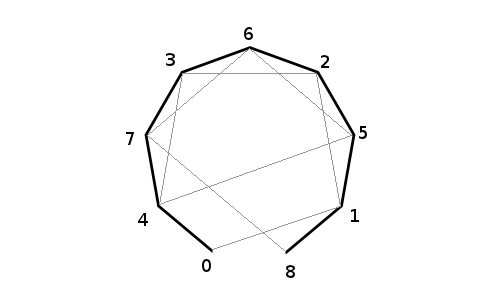
\includegraphics[scale=0.6]{images/rev_grafo_bkp.png} 
  \caption{Grafo de \bkp{} para a permutação $\pi = (~4~7~3~6~2~5~1~)$.}
  \label{fig:rev_grafo_bkp}
\end{figure}



Um ciclo em $G(\pi)$ é chamado de \textit{alternado} se as cores de
duas arestas consecutivas são diferentes ao longo do ciclo. Assim
dizemos que todos os ciclos pertencentes ao grafo serão ciclos
alternados. O \textit{comprimento} de um ciclo é a sua quantidade de
arestas pretas. Um $k$-ciclo é um ciclo que contem $k$ arestas
negras. Um \textit{ciclo longo} é um ciclo de comprimento maior que
dois.

Observe que $G(\pi)$ pode ser decomposto em ciclos de arestas
disjuntas, pois cada vertíce tem o mesmo número de arestas incidentes
cinzas e pretas. Logo existem diversas maneiras de realizar a
decomposição de ciclos em $G(\pi)$.
%..........

\subsection{Limitantes}
\label{subsec:rev_limitantes}
Para o problema de ordenação por reversões usamos os seguintes limitantes:

\begin{itemize}
\item{\textit{rev\_def}. 
Este é o limitante padrão, com limite inferior igual à $0$ e limite
superior igual a $n$ (tamanho da permutação).}
\item{\textit{rev\_br}.
Usando o conceito de \bkp{}, temos que uma reversão atua em dois
pontos em uma permutação e, portanto, pode reduzir o número de \bkp{}
em pelo menos um e no máximo dois~\cite{BafnaPevzner*1996}, levando ao
Teorema~\ref{teo:rev_bound}. 

\begin{teo}
\label{teo:rev_bound}
Para qualquer permutação $\pi$, $\frac{b_r(\pi)}{2} \leq d_r(\pi) \leq
  b_r(\pi)$.
\end{teo}
}
\item{\textit{rev\_cg}.}

\end{itemize}


\section{Ordenação por Transposições}
\label{sec:trans}
% transposicoes
Um evento de transposição ocorre quando dois blocos adjacentes no
genoma trocam de posição. Uma transposição $\rho(i, j, k)$, para
$1 \leq i < j < k \leq n + 1$, aplicada ao genoma $\pi =
(~\pi_{1}~\pi_{2}~\ldots~\pi_{n}~)$ gera a permutação $\rho\pi =
(\pi_{1}~\ldots~\pi_{i-1}~\pi_{j}~\ldots~\pi_{k-1}~\pi_{i}~\ldots$
$\pi_{j-1}~\pi_{k}~\ldots~\pi_{n})$ (Figura~\ref{fig:transposition}).

\begin{figure}[h]
  \centering
  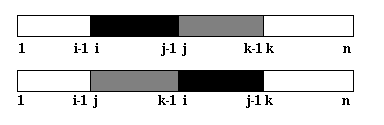
\includegraphics{images/transposition.png} 
  \caption{Transposição aplicada em uma permutação.}
  \label{fig:transposition}
\end{figure}

A distância de transposição $d_{t}(\pi, \sigma)$ entre duas
permutações $\pi$ e $\sigma$ é o número mínimo $t$ de transposições
$\rho_{1}, \rho_{2}, \ldots, \rho_{t}$ tal que
$\pi \rho_{1} \rho_{2} \ldots \rho_{t} = \sigma$. Note que a distância
de transposição entre $\pi$ e $\sigma$ é igual à distância de transposição
entre $\sigma^{-1} \pi$ e $\iota$. Então, sem perda de generalidade,
podemos dizer que o problema da distância de transposição é
equivalente ao problema de ordenação por transposições, que é a
distância de transposição entre a permutação $\pi$ e a permutação
identidade $\iota$, denotado por $d_{t}(\pi)$.

Este problema foi estudado por Bafna e
Pevzner~\cite{BafnaPevzner*1998}, onde apresentaram um algoritmo capaz
de fornecer uma resposta aproximada na razão de $1.5$, além de derivar
um importante limitante inferior para o problema. Introduziram o
conceito de \bkp{} em eventos de transposições, elementos adjacentes
em um genoma, mas não no outro, e o conceito de grafo de ciclos, ambos
ferramentas importantes utilizadas para encontrar limitantes para o
problema. Foram apresentados várias questões em aberto como verificar
a complexidade do problema da distância de transposição e o diâmetro,
que é a maior distância possível entre duas permutações de tamanho
$n$. O problema do diâmetro foi estudado por Meidanis, Walter e
Dias~\cite{MeidanisWalterDias*1997}.

A complexidade deste problema ficou em aberto por um longo tempo. O
trabalho de Bulteau, Fertin e Rusu~\cite{BulteauFertinRusu*2010}
apresentou a prova de que o problema de ordenação por transposição
pertence a classe dos problemas NP-Difíceis. Elias e
Hartman~\cite{EliasHartman*2006} apresentaram um algoritmo de
aproximação na razão de $1.375$. O trabalho de
Labarre~\cite{Labarre*2006} apresentou novos limitantes, além de
definir classes de permutações em que a distância de transposição pode
ser calculada em tempo e espaço lineares.

Nas subseções~\ref{subsec:trans_bkp} e~\ref{subsec:trans_cycle_graph}
apresentam ferramentas usadas para encontrar limitantes para o
problema de ordenação por transposições. Os limitantes usados neste
projeto estão descritos na subseção~\ref{subsec:trans_limitantes}.

\subsection{Breakpoints}
\label{subsec:trans_bkp}
No problema de ordenação por transposições, um \bkp{} é um par
$(\pi_{i}, \pi_{i+1})$ tal que $\pi_{i+1} \neq \pi_{i} + 1$. Denota-se
por $b_{t}(\pi)$ como sendo o número de \bkp{} na permutação $\pi$.

\subsection{Grafo de ciclos}
\label{subsec:trans_cycle_graph}
O conceito de grafo de ciclos foi introduzido por Bafna e
Pevzner~\cite{BafnaPevzner*1998} e foi usado para obter limitantes
melhores para o problema.

Um grafo direcionado com arestas coloridas, denotado por $G(\pi)$, é
chamado de grafo de ciclos da permutação $\pi$ se possui um conjunto
de vértices $\{0,~1,~\ldots~,~n+1\}$ e seu conjunto de arestas é
definido como para todo $1 \leq i \leq n+1$, arestas cinzas são
direcionadas de $i-1$ para $i$ e arestas pretas de $\pi_{i}$ para
$\pi_{i-1}$. A Figura~\ref{fig:trans_cycle_graph} mostra o grafo de
ciclos para a permutação $\pi = (~4~7~3~6~2~5~1~)$.

\begin{figure}[h]
  \centering 
  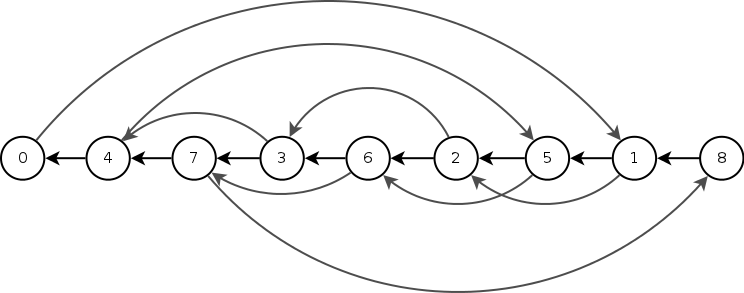
\includegraphics[scale=0.6]{images/trans_cycle_graph.png} 
  \caption{Grafo de ciclos para a permutação $\pi = (~4~7~3~6~2~5~1~)$.}
  \label{fig:trans_cycle_graph}
\end{figure}

\subsection{Limitantes}
\label{subsec:trans_limitantes}
Para o problema de ordenação por transposições usamos três tipos de
limitantes:

\begin{itemize}
\item{\textit{tra\_def}. 
Este é o limitante padrão, com limite inferior igual à $0$ e limite
superior igual a $n$ (tamanho da permutação).}
\item{\textit{tra\_br}.
Usando o conceito de \bkp{} em transposições, sabemos que uma
transposição atua em três pontos de uma permutação, logo, pode reduzir
o número de \bkp{} em pelo menos um e no máximo
três~\cite{BafnaPevzner*1998}, levando ao
Teorema~\ref{teo:trans_br_bound}.

\begin{teo}
  \label{teo:trans_br_bound}
  Para qualquer permutação $\pi$, $\frac{b_t(\pi)}{3} \leq d_t(\pi) \leq
  b_t(\pi)$.
\end{teo}
}
\item{\textit{tra\_cg}.
Usando o conceito de grafo de ciclos, um ciclo alternado de $G(\pi)$ é
ciclo direcionado com arestas de cores alternadas. Para todo vértice
de $G(\pi)$ toda aresta chegando é unicamente pareada com uma aresta
saindo de cor diferente. Isto implica que existe uma decomposição
única de ciclos alternados do conjunto de arestas de $G(\pi)$. A
seguir o termo ciclo é usado no lugar de ciclos alternados e usamos o
termo $k-\text{ciclo}$ para definir um ciclo alternado de tamanho $2k$,
$k-\text{ciclo}$ é longo se $k > 2$, e curto caso contrário.

Para melhorar o limitante, Bafna e Pevzner~\cite{BafnaPevzner*1998}
estudou separadamente os ciclos pares e ímpares. Um ciclo é impar se
número ímpar de arestas pretas e par caso contrário. Seja
$c_{ímpar}(\pi)$ o número de ciclos ímpares de $G(\pi)$, para uma
permutação $\pi$, e $\Delta c_{ímpar} (\rho) = c_{ímpar} (\pi \rho) -
c_{ímpar} (\pi)$ a mudança no número de ciclos ímpares devido a
transposição $\rho$, temos que $\Delta c_{ímpar} \in \{2, 0, -2\}$,
gerando o resultado do Teorema~\ref{teo:trans_cg_bound}.

\begin{teo} 
  \label{teo:trans_cg_bound} 
  Para qualquer permutação $\pi$, $\frac{n + 1 - c_{ímpar}(\pi)}{2} \leq
  d_t(\pi) \leq \frac{3}{4} (n + 1 - c_{ímpar}(\pi))$.
\end{teo}
}
\end{itemize}


\section{Ordenação por Reversões e Transposições}
\label{sec:rev_trans}
% reversoes e transposicoes
Na natureza um genoma não sofre apenas eventos de reversão ou de
transposição, ele está exposto a diversos eventos diferentes. Para
esta situação, iremos estudar o caso onde os eventos de reversão e
transposição ocorrem simultaneamente sobre um genoma.

A distância de reversão e transposição $d_{rt}(\pi, \sigma)$ entre
duas permutações $\pi$ e $\sigma$ é o número mínimo $rt$ de reversões
e transposições $\rho_{1}, \rho_{2}, \ldots, \rho_{rt}$ tal que
$\pi \rho_{1} \rho_{2} \ldots \rho_{rt} = \sigma$. Como no caso em que
os eventos ocorrem individualmente, podemos dizer, sem perda de
generalidade, que o problema da distância de reversão e transposição é
equivalente ao problema de ordenação por reversões e transposições,
que é a distância de reversão e transposição entre a permutação $\pi$ e a
permutação identidade $\iota$, denotado por $d_{rt}(\pi)$.




\chapter{Modelos}
\label{cap:model}
%%%%%%%%%%%%%%%%%%%%%%%%%%%%%%%%%%%%%%%%
% COLOCAR AS REFERENCIAS DO CAPITULO 2 %
% EXPLICAR BOTTOM-UP                   %
%%%%%%%%%%%%%%%%%%%%%%%%%%%%%%%%%%%%%%%%
Neste capítulo nós apresentaremos a descrição dos modelos de \pr{} e
\pli{} usados para os problemas de ordenação por transposições,
ordenação por reversões e ordenação por reversões e transposições.

\section{\PR}
\label{sec:cp}
O modelo de \pr{} usado para o problema de ordenação por transposições
é o descrito em Dias e Dias~\cite{DiasDias*2009}. Nós usamos os
limitantes inferior e superior descritos em (??) para escrever as
formulações baseadas nas teorias de Problema de Satisfação de
Restrições (CSP) e Problema de Otimização com Restrições (COP). As
formulações foram descritas usando a notação prolog-like de
Marriot \cite{Marriott*1998}. Primeiramente iremos apresentar os
predicados que são comum às duas formulações.

Em prolog as variáveis são descritas por \textit{strings} iniciadas
com letra maiúscula ou ``\_'' (\textit{underscore}) caso a variável
seja anônima. As letras gregas $\pi$ e $\sigma$ representam listas
nesta notação. A construção $X~::~[i~..~j]$ significa que $X$ (ou cada
elemento de $X$ se $X$ for uma lista) pode assumir um valor do
intervalo $[i~..~j]$.

A representação da permutação (\ref{perm}) e o efeito das operações de
reversão (\ref{reversal}) e transposição (\ref{transposition} podem
ser vistas da mesma maneira que são descritas pelos problemas. Neste
modelo a permutação $\pi$ é uma lista de elementos
($\pi_{1},~\pi_{2},~\ldots~,~\pi_{n}$) onde $\pi_{i} \in \mathbb{N}$,
$0 < \pi_{i} \le n$ e $\pi_{i} \neq \pi_{j}$ para $i \neq j$.
\begin{align}
  \label{perm}
  \begin{split}
  \textit{per}&\textit{mutation}(\pi, N)~\text{:-} \\
  &\textit{length}(\pi, N), \\ 
  &\pi~::~[1~..~N], \\
  &\textit{all\_different}(\pi). 
  \end{split}
\end{align}

Na reversão $\rho(i,j)$, $0 < i < j \leq n$, dividimos a lista em três
sublistas $C_{1}C_{2}C_{3}$ onde $C_{1} = (\pi_{1}~..~\pi_{i-1})$,
$C_{2} = (\pi_{i}~..~\pi_{j})$ e $C_{3} =
(\pi_{j+1}~..~\pi_{n})$. Depois fazemos a reversão na sublista
$C_{2}$, resultando na lista $R_{C_{2}}$. Então juntamos a nova lista
$R_{C_{2}}$ com as sublistas $C_{1}$ e $C_{3}$ para formar $\rho\pi =
C_{1}R_{C_{2}}C_{3}$.
\begin{align}
  \label{reversal}
  \begin{split}
  \textit{rev}&\textit{ersal}(\pi, \sigma, I, J)~\text{:-} \\
  &\textit{permutation}(\pi, N), \\
  &\textit{permutation}(\sigma, N),  \\
  &1 \le I < J \le N, \\
  &\textit{split}(\pi, I, J, C_{1}, C_{2}, C_{3}), \\
  &\textit{reverse}(C_{2}, R_{C_{2}}),  \\
  &\sigma = C_{1}, R_{C_{2}}, C_{3}. 
  \end{split}
\end{align}

Na transposição $\rho(i,j,k)$, $0 < i < j < k\leq n$, dividimos a
lista em quatro sublistas $C_{1}C_{2}C_{3}C_{4}$ onde $C_{1} =
(\pi_{1}~..~\pi_{i-1})$, $C_{2} = (\pi_{i}~..~\pi_{j-1})$, $C_{3} =
(\pi_{j}~..~\pi_{k-1})$ e $C_{4} = (\pi_{k}~..~\pi_{n})$. Trocamos de
posição os blocos $C_{2}$ e $C_{3}$ e juntamos elas na ordem $C_{1}$,
$C_{3}$, $C_{2}$ e $C_{4}$ para formar $\rho\pi =
C_{1}C_{3}C_{2}C_{4}$. Observe que as sublistas $C_{1}$ e $C_{4}$
podem ser vazias.
\begin{align}
  \label{transposition}
  \begin{split}
  \textit{tra}&\textit{nsposition}(\pi, \sigma, I, J, K)~\text{:-} \\
  &\textit{permutation}(\pi, N), \\
  &\textit{permutation}(\sigma, N), \\
  &1 \le I < J < K \le N,  \\
  &\textit{split}(\pi, I, J, K, C_{1}, C_{2}, C_{3}, C_{4}), \\
  &\sigma = C_{1}, C_{3}, C_{2}, C_{4}. 
  \end{split}
\end{align}

\subsection{Modelo CSP}
\label{subsec:modelcsp}
Primeiramente modelaremos o problema usando a teoria CSP, mas o número
de variáveis é desconhecido devido ao fato de precisarmos do valor da
distância $d_{r}(\pi)$ para criar as restrições e variáveis que
representam as permutações. Por esta razão, nós escolhemos um valor
candidato para a distância $R$ tal que $R \in [LB~..~UB]$, onde $LB$ é
um limitante inferior conhecido e $UB$ é um limitante superior
conhecido para o problema, e tentamos achar uma combinação apropriada
de $R$ reversões que solucionam o problema. Se o modelo CSP falha (não
existe combinação que soluciona o problema com o valor candidato
escolhido) com o candidato $R$, nós escolhemos outro valor $R$ apenas
incrementando seu valor. O valor de $R$ é escolhido usando uma
estratégia \textit{bottom-up}\footnote{EXPLICAR BOTTOM-UP} e por
definição não verificamos nenhum valor maior que o limitante superior
$UB$. Na transposição, o processo é o mesmo que na reversão, trocando
apenas o valor da distância de reversão ($d_{r}(\pi)$) para o valor da
distância de transposição ($d_{t}(\pi)$).
\begin{align}
  \label{revdistance}
  \begin{split}
  \textit{rev}&\textit{ersal\_distance}(\iota, 0, \_Model). \\
  \textit{rev}&\textit{ersal\_distance}(\pi, R, Model)~\text{:-} \\
  &\textit{bound}(\pi, Model, LB, UB), \\
  &R :: [LB~..~UB], \\
  &\textit{indomain}(R),  \\
  &\textit{reversal}(\pi, \sigma, \_I, \_J),  \\
  &\textit{reversal\_distance}(\sigma, R-1, Model). 
  \end{split}
\end{align}
\begin{align}
  \label{tradistance}
  \begin{split}
  \textit{tra}&\textit{nsposition\_distance}(\iota, 0, \_Model). \\
  \textit{tra}&\textit{nsposition\_distance}(\pi, T, Model)~\text{:-} \\
  &\textit{bound}(\pi, Model, LB, UB), \\
  &T :: [LB~..~UB], \\
  &\textit{indomain}(T),  \\
  &\textit{transposition}(\pi, \sigma, \_I, \_J, \_K),  \\
  &\textit{transposition\_distance}(\sigma, T-1, Model). 
  \end{split}
\end{align}

O predicado \textit{rev\_trans\_dist/3} (\ref{trarevdist}) retorna o
valor da distância de reversão e transposição. O
predicado \textit{event/2} escolhe o melhor evento entre o
predicado \textit{reversal/4} (\ref{reversal}) e o
predicado \textit{transposition/5} (\ref{transposition}) para
minimizar o valor da distância.
\begin{align}
  \label{trarevdist}
  \begin{split}
  \textit{rev}&\textit{\_trans\_dist}(\iota, 0, \_Model). \\
  \textit{rev}&\textit{\_trans\_dist}(\pi, N, Model)~\text{:-} \\
  &\textit{bound}(\pi, Model, LB, UB), \\
  &N :: [LB~..~UB], \\
  &\textit{indomain}(N),  \\
  &\textit{event}(\pi, \sigma),  \\
  &\textit{rev\_trans\_dist}(\sigma, N-1, Model). 
  \end{split}
\end{align}

O predicado \textit{indomain(X)} em (\ref{revdistance}),
(\ref{tradistance}) e (\ref{trarevdist}) pega o domínio da variável
$X$ e escolhe o menor elemento dele (no caso o valor do limitante
inferior). Se o modelo retorna para o predicado \textit{indomain}
devido a uma falha, o elemento que originou ela será removido do
domínio e um outro valor será escolhido.

Os modelos CSP para os problemas possuem a estrutura mostrada acima,
trocando apenas os limitantes usados. Em comum a todas operações temos
o modelo \textit{def\_csp} que não usa nenhum limitante.

\textit{Ordenação por reversões:}
\begin{itemize}
\item{\textit{rev\_br\_csp}: 
Modelo que usa o conceito de \bkp{} em reversões para calcular os
limitantes descritos no Teorema~\ref{teo:rev_bkp_bound}.}
\item{\textit{rev\_cg\_csp}:
Modelo que usa o número de $2$-ciclos na máxima decomposição em ciclos
de $G(\pi)$ para calcular os limitantes descritos no
Teorema~\ref{teo:rev_cic_bound}.}
\end{itemize}

\textit{Ordenação por transposições:}
\begin{itemize}
\item{\textit{tra\_br\_csp}: 
Modelo que usa o conceito de \bkp{} em transposições para calcular os
limitantes conforme descrito .... (??)}
\item{\textit{tra\_cg\_csp}:
Modelo que usa o conceito de grafo de ciclos em transposições, fazendo
a decomposição de ciclos e analisando os ciclos ímpares separadamente
para calcular os limitantes conforme descrito .... (??)}
\end{itemize}

\textit{Ordenação por reversões e transposições:} 
\begin{itemize}
\item{\textit{r\_t\_br\_csp}: 
Melhor limitante superior entre o limitante de \bkp{} para reversões e
o limitante de \bkp{} para transposições.}
\item{\textit{r\_t\_bc\_csp}:
Melhor limitante superior entre o limitante de \bkp{} para reversões e
o limitante do grafo de ciclos para transposições.}
\item{\textit{r\_t\_cc\_csp}: 
Melhor limitante superior entre o limitante do grafo de ciclos para
reversões e o limitante do grafo de ciclos para transposições.}
\end{itemize}

O predicado \textit{bound/4} (\ref{bound}) recebe na
variável \textit{Model} um átomo que representa o modelo a ser
usado. Este átomo se conecta com o predicado que retorna o limitante
superior e inferior apropriado para o modelo. Observe que o limitante
inferior é igual a $0$ no caso dos modelos de ordenação por reversões
e transposições. Isto ocorre devido ao fato que a cada nova iteração
do modelo pode surgir um limitante inferior melhor, simplesmente
fazendo a troca entre as operações de reversão e transposição.
\begin{align}
  \label{bound}
  \begin{split}
  \textit{bou}&\textit{nd}(\pi, def\_csp, LB, UB)~\text{:-} \\
  &\textit{def\_csp\_bound}(\pi, LB, UB).  \\
  \textit{bou}&\textit{nd}(\pi, rev\_br\_csp, LB, UB)~\text{:-}  \\
  &\textit{calc\_breakpoints\_reversal}(\pi, B), \\
  &LB = B / 2  \\ % / 2 ,  \\
  &UB = B.  \\
  \textit{bou}&\textit{nd}(\pi, rev\_cg\_csp, LB, UB)~\text{:-}  \\
  &\textit{find\_2\_cycle}(\pi, B, C), \\
  &LB = (2 * B - C) / 3 ,   \\
  &UB = B - C / 2.  \\
  \textit{bou}&\textit{nd}(\pi, tra\_br\_csp, LB, UB)~\text{:-} \\
  &\textit{calc\_breakpoints\_transposition}(\pi, B), \\
  &LB = B / 3  \\ %/ 3,  \\
  &UB = B.   \\
  \textit{bou}&\textit{nd}(\pi, tra\_br\_csp, LB, UB)~\text{:-} \\
  &\textit{calc\_oddcycle\_transposition}(\pi, N, C), \\
  &LB = (N + 1 - C) / 2  \\ 
  &UB = (3 * (N + 1 - C)) / 4.  \\
  \textit{bou}&\textit{nd}(\pi, r\_t\_br\_csp, 0, UB)~\text{:-} \\
  &\textit{bound}(\pi, rev\_br, \_RLB, RUB), \\
  &\textit{bound}(\pi, tra\_br, \_TLB, TUB), \\
  &\textit{min}(RUB, TUB, UB), \\
  \textit{bou}&\textit{nd}(\pi, r\_t\_bc\_csp, 0, UB)~\text{:-} \\
  &\textit{bound}(\pi, rev\_br, \_RLB, RUB), \\
  &\textit{bound}(\pi, tra\_cg, \_TLB, TUB), \\
  &\textit{min}(RUB, TUB, UB), \\
  \textit{bou}&\textit{nd}(\pi, r\_t\_cc\_csp, 0, UB)~\text{:-} \\
  &\textit{bound}(\pi, rev\_cg, \_RLB, RUB), \\
  &\textit{bound}(\pi, tra\_cg, \_TLB, TUB), \\
  &\textit{min}(RUB, TUB, UB), 
  \end{split}
\end{align}

\subsection{Modelo COP}
\label{subsec:modelcop}
Uma outra alternativa é modelar o problema usando a teoria COP. Os
modelos que usam esta abordagem necessitam de um limitante superior,
portanto serão feitas algumas alterações nos predicados definidos
anteriormente. Nós usamos as variáveis binárias $B$ para indicar
quando uma operação de reversão ou de transposição modificou ou não a
permutação fornecida.

O primeiro predicado que precisamos criar é o \textit{reversal\_cop/5}
(\ref{reversal_cop}). Primeiramente, dado uma reversão $\rho(i, j)$,
adicionamos uma nova restrição para permitir $(i, j) = (0, 0)$. Se
$(i, j) = (0, 0)$ então $\pi\rho = \pi$. Então, adicionamos um novo
argumento ao predicado \textit{reversal\_cop} que recebe a variável
$B$.
\begin{align}
  \label{reversal_cop}
  \begin{split}
  \textit{rev}&\textit{ersal\_cop}(\iota, \iota, 0, 0, 0). \\
  \textit{rev}&\textit{ersal\_cop}(\pi, \sigma, I, J, 1)~\text{:-}~ 
  \textit{reversal}(\pi, \sigma, I, J).
  \end{split}
\end{align}

O predicado equivalente para transposição é
o \textit{transposition\_cop/6} (\ref{transposition_cop}). Neste caso,
dado uma transposição $\rho(i, j, k)$, adicionamos uma nova restrição
para permitir $(i, j, k) = (0, 0, 0)$. Se $(i, j, k) = (0, 0, 0)$
então $\pi\rho = \pi$.
\begin{align}
  \label{transposition_cop}
  \begin{split}
  \textit{tra}&\textit{nsposition\_cop}(\iota, \iota, 0, 0, 0, 0). \\
  \textit{tra}&\textit{nsposition\_cop}(\pi, \sigma, I, J, K, 1)~\text{:-}~ 
  \textit{transposition}(\pi, \sigma, I, J, K). 
  \end{split}
\end{align}

Para calcular a distância nos modelos baseados na teoria COP,
implementamos o predicado \textit{reversal\_distance\_cop/3}
(\ref{revdistance_cop}), que ajusta as variáveis $B$ usando o valor do
limitante superior e restringe as permutações fazendo $\pi_{k}
= \pi_{k-1} \rho_{k}$. O predicado \textit{length/2}, predicado
interno do prolog, é usado para criar uma lista de variáveis não
instanciadas com o tamanho dado. A função de custo \textit{Cost} é a
soma das variáveis $B$ associadas com cada $\rho_{k}$, $Cost
= \sum_{k=1}^{UB} B_{k}$, onde $UB$ é um limitante superior
conhecido. A distância de reversão é o valor mínimo da função de custo
$d_{r} = \min Cost$. Para evitar processamento desnecessários, o valor
de $Cost$ precisa ser maior ou igual a qualquer limitante inferior. O
predicado equivalente para transposição é
o \textit{transposition\_distance\_cop/3} (\ref{tradistance_cop}).
\begin{align}
  \label{revdistance_cop}
  \begin{split}
  \textit{rev}&\textit{ersal\_distance\_cop}(\pi, R, Model)~\text{:-} \\
  &\textit{bound}(\pi, Model, LB, UB), \\
  &\textit{length}(B, UB),  \\
  &\textit{upperbound\_constraint\_rev}(\pi, B, Model, UB), \\
  &\textit{sum}(B, Cost),  \\
  &\textit{Cost} \ge \textit{LB},  \\
  &\textit{minimize}(Cost, R). 
  \end{split}
\end{align}
\begin{align}
  \label{tradistance_cop}
  \begin{split}
  \textit{tra}&\textit{nsposition\_distance\_cop}(\pi, T, Model)~\text{:-} \\
  &\textit{bound}(\pi, Model, LB, UB), \\
  &\textit{length}(B, UB),  \\
  &\textit{upperbound\_constraint\_trans}(\pi, B, Model, UB), \\
  &\textit{sum}(B, Cost),  \\
  &\textit{Cost} \ge \textit{LB},  \\
  &\textit{minimize}(Cost, T). 
  \end{split}
\end{align}

O predicado equivalente para o modelo de ordenação por reversões e
transposições é
o \textit{rev\_trans\_dist\_cop/3}~(\ref{trarevdistcop}). O
predicado \textit{upperbound\_constraint\_event/4} escolhe o melhor
evento entre a reversão, usando o
predicado \textit{upperbound\_constraint\_rev/4}
(\ref{ub_constaint_rev}), e a transposição, usando o
predicado \textit{upperbound\_constraint\_trans/4}
(\ref{ub_constaint_tra}), para minimizar o valor da distância.
\begin{align}
  \label{trarevdistcop}
  \begin{split}
  \textit{rev}&\textit{\_trans\_dist\_cop}(\pi, N, Model)~\text{:-} \\
  &\textit{bound}(\pi, Model, LB, UB), \\
  &\textit{length}(B, UB),  \\
  &\textit{upperbound\_constraint\_event}(\pi, B, Model, UB), \\
  &\textit{sum}(B, Cost),  \\
  &\textit{Cost} \ge \textit{LB},  \\
  &\textit{minimize}(Cost, N). 
  \end{split}
\end{align}

O predicado \textit{upperbound\_constraint\_rev/4}
(\ref{ub_constaint_rev}) aplica na permutação os efeitos de $\rho_{k}$
e retorna o valor apropriado de $B$ para cada reversão $\rho_{k}$. Uma
restrição importante é verificar se é possível ordenar a permutação
usando o número restante de reversões para evitar processamento
desnecessário. O predicado equivalente para a transposição é o
\textit{upperbound\_constraint\_trans/4} (\ref{ub_constaint_tra}).
\begin{align}
  \label{ub_constaint_rev}
  \begin{split}
  \textit{upp}&\textit{erbound\_constraint\_rev}(\iota, [~], \_Model, \_UB). \\
  \textit{upp}&\textit{erbound\_constraint\_rev}(\pi, [B|Bt], Model, UB)~\text{:-} \\
  &\textit{reversal\_cop}(\pi, \sigma, \_I, \_J, B), \\
  &\textit{bound}(\pi, Model, LB, \_UB), \\
  &UB \ge LB,  \\
  &\textit{upperbound\_constraint\_rev}(\sigma, Bt, Model, UB - 1),  
  \end{split}
\end{align}
\begin{align}
  \label{ub_constaint_tra}
  \begin{split}
  \textit{upp}&\textit{erbound\_constraint\_trans}(\iota, [~], \_Model, \_UB). \\
  \textit{upp}&\textit{erbound\_constraint\_trans}(\pi, [B|Bt], Model, UB)~\text{:-} \\
  &\textit{transposition\_cop}(\pi, \sigma, \_I, \_J, \_K, B), \\
  &\textit{bound}(\pi, Model, LB, \_UB), \\
  &UB \ge LB,  \\
  &\textit{upperbound\_constraint\_trans}(\sigma, Bt, Model, UB - 1),  
  \end{split}
\end{align}

Os modelos baseados na teoria COP possuem a estrutura acima, trocando
apenas os limitantes usados. Os limitantes são os mesmos usados para
os modelos CSP, modificados para os modelos COP. Então temos os
seguintes limitantes: \textit{def\_cop}, \textit{rev\_br\_cop},
\textit{rev\_cg\_cop}, \textit{tra\_br\_cop}, \textit{tra\_cg\_cop}, 
\textit{r\_t\_br\_cop}, \textit{r\_t\_bc\_cop}
e \textit{r\_t\_cc\_cop}.

\section{\PLI}
\label{sec:pli}
A abordagem utilizada para programação linear inteira é a descrita no
trabalho de Dias e de Souza~\cite{DiasSouza*2007}. Neste trabalho,
define-se um modelo para o problema da distância com tamanho
polinomial em relação ao tamanho da permutação fornecida como
entrada. O modelo é específico para os eventos de reversão,
transposição ou reversão e transposição quando ocorrem
simultaneamente.

Primeiramente vamos apresentar as variáveis e restrições que são
comuns para todos os modelos. A ideia é assegurar que só estamos
tratando com permutações válidas.

\textit{Gerando permutações válidas a cada iteração.} 
As variáveis $B_{ijk}$ indicam se a $i$-ésima posição de $\pi$ possui
o valor $j$ depois da $k$-ésima operação ter sido executada, para todo
$1 \le i, j \le n$ e todo $ 0 \le k < n$.

\[ 
B_{ijk} = \left \{ 
\begin{tabular}{ll} 
  1, & se $\pi[i]$ = $j$ depois da $k$-ésima operação \\ 
  0, & caso contrário
\end{tabular} 
\right .
\]

As restrições (\ref{eq:corr1}) e (\ref{eq:corr2}) garantem que a
permutação inicial e a final são corretas. 
\begin{align} 
  B_{i,\pi[i],0} = 1,~\text{para todo $1 \le i \le n$}. \label{eq:corr1} \\
  B_{i,\sigma[i],n-1} = 1,~\text{para todo $1 \le i \le n$}. \label{eq:corr2}
\end{align}

A restrição (\ref{eq:posval}) garante que cada posição de uma
permutação possui exatamente um valor associado a ela. Já a restrição
(\ref{eq:valpos}) garante que todo valor esteja associado a uma
posição de cada permutação.
\begin{align}
  \sum_{j=1}^{n} B_{ijk} = 1,~\text{para todo $1 \le i \le n$, 
  $0 \le k < n$}. \label{eq:posval} \\
  \sum_{i=1}^{n} B_{ijk} = 1,~\text{para todo $1 \le j \le n$, $0 \le
   k < n$}. \label{eq:valpos}
\end{align}

\textit{Distância de reversão.}
Para o problema da distância de reversão definimos os seguintes
conjuntos de variáveis e restrições. As variáveis binárias $r_{abk}$
indicam quando a $k$-ésima operação de reversão afeta o blocos
$\pi[a~\ldots~b]$ de $\pi$, para todo $1 \le a < b \le n$ e todo
$1 \le k < n$.

\[
r_{abk} = \left \{ 
\begin{tabular}{ll} 
  1, & se $\rho_{k} = \rho(a,b)$ \\
  0, & caso contrário
\end{tabular} 
\right .
\]

As variáveis binárias $r_{k}$ são usadas para decidir se a $k$-ésima
operação de reversão modificou a permutação, para todo $ 1 \le k < n$.

\[
r_{k} = \left \{ 
\begin{tabular}{ll} 
 1, & se $\rho_{k} = \rho(x,y)$ e
 $\rho_{k} \rho_{k-1}~\ldots~\rho_{1} \pi \neq \rho_{k-1}~\ldots~\rho_{1} \pi$\\
 0, & caso contrário 
\end{tabular}
\right .
\]

As restrições (\ref{eq:rev1}) e (\ref{eq:rev2}) são necessárias para
identificar as reversões que fazem parte da solução. A restrição
(\ref{eq:rev1}) garante que se a $k$-ésima reversão não alterar a
permutação, nenhuma das reversões seguintes poderá alterar. Já a
restrição (\ref{eq:rev2}) garante que no máximo uma reversão poderá
ser feita por iteração.
\begin{align}
  &r_{k} \le r_{k-1},~\text{para todo $1 \le k <
  n$}. \label{eq:rev1} \\
  \sum_{a=1}^{n-1}\sum_{b=a+1}^{n}
  &r_{abk} \le r_{k},~\text{para todo $1 \le k < n$}. \label{eq:rev2}
\end{align}

As próximas restrições lidam com as modificações na permutação causada
pela reversão a cada iteração da execução. A análise será dividida em
dois casos onde, para cada caso, analisamos cada posição $i$ da
permutação para verificar seu valor após a operação de reversão
$\rho(a,b)$ ser completada.
\begin{enumerate}
\item{$i < a$ ou $i > b$:
A operação de reversão não modifica estas posições.
\begin{align}
  \begin{split}
    \sum_{a=i+1}^{n-1}\sum_{b=a+1}^{n} r_{abk} +
    \sum_{a=1}^{n-1}\sum_{b=a+1}^{i-1} r_{abk} +
    (1 - r_{k}) + B_{i,j,k-1} - B_{ijk} \le 1, \\
    \text{para todo $1 \le i,~j \le n$ e todo $1 \le k < n$}.
  \end{split}
  \label{eq:rev3}
\end{align}}
\item{$a \le i \le b$:
A operação de reversão altera os elementos guardados nestas
posições. Para não ser redundante, a desigualdade precisa ter os dois
primeiros termos com valor $1$. Neste caso, $B_{b+a-i,j,k-1} = 1$,
implicando que o elemento $j$ foi salvo na posição $b + a - i$ antes
da reversão ser movida para a posição $i$ ($B_{ijk} = 1$).
\begin{align}
  \begin{split}
  r_{abk} + B_{b+a-i,j,k-1} - B_{ijk} \le 1, \\
  \text{$1 \le a < b \le n,~a \le i \le b,~1 \le j
    \le n,~1 \le k < n$}.
  \end{split}
  \label{eq:rev4}
\end{align}}
\end{enumerate}

\textit{Distância de transposição.}
Para o problema da distância de transposição, usaremos os seguintes
conjuntos de variáveis e restrições. As variáveis binárias $t_{abck}$
indicam quando a $k$-ésima operação de transposição realiza a troca de
lugares dos blocos $\pi[a~\ldots~b - 1]$ e $\pi[b~\ldots~c - 1]$ da
permutação $\pi$, para todo $1 \le a < b < c \le n + 1$ e todo $ 1 \le
k < n$.

\[ 
  t_{abck} = \left \{ 
  \begin{tabular}{ll} 
  1, & se $\rho_{k} = \rho(a,b,c)$ \\ 
  0, & caso contrário 
  \end{tabular} \right .
\] 

As variáveis binárias $t_{k}$ são usadas para decidir se a $k$-ésima
operação de transposição modificou a permutação, para todo $ 1 \le k <
n$.

\[ 
  t_{k} = \left \{ 
  \begin{tabular}{ll} 
  1, & se $\rho_{k} = \rho(x,y,z)$ e
  $\rho_{k} \rho_{k-1}~\ldots~\rho_{1} \pi \neq \rho_{k-1}~\ldots~\rho_{1} \pi$\\
  0, & caso contrário 
  \end{tabular} \right .
\]

As restrições (\ref{eq:transp1}) e (\ref{eq:transp2}) são necessárias
para identificar as transposições que fazem parte da solução. A
restrição (\ref{eq:transp1}) garante que se a $k$-ésima transposição
não alterar a permutação, nenhuma das transposições seguintes poderá
alterar. Já a restrição (\ref{eq:transp2}) garante que no máximo uma
transposição poderá ser feita por iteração.
\begin{align}
  &t_{k} \le t_{k-1}, \text{para todo $1 \le k <
  n$}. \label{eq:transp1} \\
  \sum_{a=1}^{n-1}\sum_{b=a+1}^{n}\sum_{c=b+1}^{n+1} &t_{abck} \le
  t_{k} , \text{para todo $1 \le k <
  n$}. \label{eq:transp2} 
\end{align}

As próximas restrições refletem a modificações na permutação causada
por uma transposição a cada passo da execução. A análise será dividida em
três casos onde, para cada caso, analisamos cada posição $i$ da
permutação para verificar seu valor após a operação de transposição
$\rho(a,b,c)$ ser completada.
\begin{enumerate}
\item{$i < a$ ou $i \ge c$:
A operação de transposição não altera estas posições.
\begin{align}
  \begin{split} 
    \sum_{a=i+1}^{n-1}\sum_{b=a+1}^{n}\sum_{c=b+1}^{n+1} t_{abck}
    + \sum_{a=1}^{n-1}\sum_{b=a+1}^{n}\sum_{c=b+1}^{i} t_{abck} + (1 -
    t_{k}) + B_{i,j,k-1} - B_{ijk} \le 1, \\
    \text{para todo $1 \le i, j \le n$ e todo $1 \le k <
    n$}.
  \end{split} \label{eq:transp3}
\end{align}}
\item{$a \le i < a + c -b$:
Após a operação de transposição ser completada, estas posições serão
ocupadas pelos elementos que estão nas posições de $b$ a $c - 1$. Para
não ser redundante, esta desigualdade precisa ter os dois primeiros
termos com o valor $1$. Neste caso, temos que $B_{b-a+i,j,k-1} = 1$,
implicando que o elemento $j$ foi salvo na posição $b - a + i$ antes
da transposição ser movida para a posição $i$ ($B_{ijk} = 1$).
\begin{align}
  \begin{split}
  t_{abck} + B_{b-a+i,j,k-1} - B_{ijk} \le 1, \\
  \text{$1 \le a < b < c \le n + 1, a \le i < a + c -b, 1 \le j
  \le n, 1 \le k < n$}.
  \end{split}
  \label{eq:transp4}
\end{align}}
\item{$a + c - b \le i < c$:
Após a operação de transposição ser completada, estas posições serão
ocupadas pelos elementos que estão nas posições de $a$ a $b -
1$. Similar com o caso acima, esta desigualdade é redundante se os
valores dos dois primeiros termos não for igual a $1$. Isto significa
que a $k$-ésima transposição move $B^{k-1}[a~..~b-1]$ para as posições
que precedem a posição $c$. Por definição, $i$ representa uma das
posições que receberão um elemento deste subvetor. Então, temos que
$B^{k}[i] = B^{k-1}[b - c + i]$, para todo $i \in [a + c - b~..~c -
1]$ e os últimos dois termos se anulam.
\begin{align}
  \begin{split}
  t_{abck} + B_{b-c+i,j,k-1} - B_{ijk} \le 1, \\
  \text{$1 \le a < b < c \le n + 1, a + c - b \le i < c, 1 \le j
  \le n, 1 \le k < n$}.  
  \end{split}
  \label{eq:transp5}
\end{align}}
\end{enumerate}

\textit{Distância de reversão e transposição.}
Para o problema da distância de reversão e transposição usaremos todas
as variáveis definidas anteriormente, com a adição das variáveis
binárias $z_{k}$, que é usada para indicar quando uma $k$-ésima
operação, seja ela uma reversão ou uma transposição, realmente
modificou a permutação. Então, para todo $1 \le k < n$, temos que:

\[
z_{k} = \left \{ 
  \begin{tabular}{ll} 
  1, & se $\rho_{k} = \rho(x,y)$ ou $\rho_{k} = \rho(x,y,z)$ e
  $\rho_{k} \rho_{k-1}~\ldots~\rho_{1} \pi \neq \rho_{k-1}~\ldots~\rho_{1} \pi$\\
  0, & caso contrário
  \end{tabular} \right .
\]

Usaremos todas as restrições definidas anteriormente, com exceção das
restrições (\ref{eq:rev1}) e (\ref{eq:transp1}) que serão substituídas
pelas restrições (\ref{eq:rt1}) e (\ref{eq:rt2}). A restrição
(\ref{eq:rt1}) garante que se não ocorreu operações em uma iteração
então não ocorrerá nenhuma operação nas iterações seguintes. A
restrição (\ref{eq:rt2}) garante que no máximo uma operação é
executada a cada iteração.
\begin{align}
  &z_{k} \le z_{k-1}, \text{para todo $1 \le k <
    n$}. \label{eq:rt1} \\ 
  &r_{k} + t_{k} = z_{k} , \text{para todo
    $1 \le k < n$}. \label{eq:rt2}
\end{align}

Precisamos modificar as restrições (\ref{eq:rev3}) e
(\ref{eq:transp3}), substituindo $r_{k}$ e $t_{k}$ por $z_{k}$,
resultando nas restrições (\ref{eq:rt3}) e (\ref{eq:rt4}).
\begin{align}
  \begin{split}
    \sum_{a=i+1}^{n-1}\sum_{b=a+1}^{n} r_{abk} +
    \sum_{a=1}^{n-1}\sum_{b=a+1}^{i-1} r_{abk} +
    (1 - z_{k}) + B_{i,j,k-1} - B_{ijk} \le 1, \\
    \text{para todo $1 \le i,~j \le n$ e todo $1 \le k < n$}.
  \end{split} \label{eq:rt3} \\
  \begin{split} 
    \sum_{a=i+1}^{n-1}\sum_{b=a+1}^{n}\sum_{c=b+1}^{n+1} t_{abck}
    + \sum_{a=1}^{n-1}\sum_{b=a+1}^{n}\sum_{c=b+1}^{i} t_{abck} + (1 -
    z_{k}) + B_{i,j,k-1} - B_{ijk} \le 1, \\
    \text{para todo $1 \le i, j \le n$ e todo $1 \le k <
    n$}.
  \end{split} \label{eq:rt4}
\end{align}

\subsection{Função Objetivo}
\label{subsec:fo}
Considerando as variáveis e restrições descritas anteriormente para
cada um dos três problemas de distâncias, temos a função objetivo
$\omega_{r} = \min \sum_{k=1}^{n-1} r_{k}$, para o problema da
distância de reversão, a função objetivo $\omega_{t}
= \min \sum_{k=1}^{n-1} t_{k}$, para o problema da distância de
transposição, e a função objetivo $\omega_{rt} = \min \sum_{k=1}^{n-1}
z_{k}$, para o problema da distância de reversão e transposição quando
ocorrem simultaneamente.

\subsection{Tamanho do modelo}
\label{subsec:modelsize}
É fácil observar que o modelo descrito possui tamanho polinomial em
relação ao tamanho da permutação fornecida como entrada. A
tabela~\ref{table:modelsize} mostra o tamanho do modelo para os três
problemas de distâncias com relação ao parâmetro $n$ (tamanho da
permutação de entrada).

\begin{table}[h]
\caption{Tamanho dos modelos em relação à $n$.}
\label{table:modelsize}
\center
\begin{tabular}{|l|c|c|}
  \hline
  \textbf{Modelo} & \textbf{Variáveis} & \textbf{Restrições} \\
  \hline
  Distância de Reversão & $O(n^3)$ & $O(n^5)$ \\
  Distância de Transposição & $O(n^4)$ & $O(n^6)$ \\
  Distância de Reversão e Transposição & $O(n^4)$ & $O(n^6)$ \\
  \hline
\end{tabular}
\end{table}


\chapter{Análise dos Resultados}
\label{cap:resul}
% resultados
Neste capítulo apresentaremos os resultados obtidos pelos modelos
descritos no capítulo~\ref{cap:model}. A seção \ref{sec:tspec} mostra
as características do computador utilizado para executar os
testes. ---MORE HERE---. A seção \ref{sec:analise} apresenta a análise dos
resultados obtidos durante este trabalho.

\section{Especificações Técnicas}
\label{sec:tspec}
O computador utilizado para executar os testes possui as seguintes
características:

\begin{itemize}
  \item{Processador: Intel\textregistered{}~Core\texttrademark~2 Duo
  2.33GHz.}

  \item{Memória RAM: 3 GB.}
  
  \item{Sistema Operacional: Ubuntu Linux com kernel 2.6.31.}
\end{itemize}

Todos modelos de \pr{} foram implementados usando as seguintes
ferramentas:

\begin{itemize}
  \item{Sistema de programação de código
  aberto \textit{ECLiPSe-6.0}~\cite{eclipse*2009}. } 
  
 \item{Pacote proprietário para a linguagem de programação
  C++ \textit{IBM\textregistered{} ILOG\textregistered{}
  CPLEX\textregistered{} CP Optimizer v 2.3}~\cite{ilogcp*2011}.}
\end{itemize}

Todas formulações de programação linear inteira foram implementadas
usando as seguintes ferramentas:

\begin{itemize}
  \item{Sistema de programação de código
  aberto \textit{GLPK-4.35}~\cite{glpk*2010}.}
  
  \item{Pacote proprietário para a linguagem de programação
  C++ \textit{IBM\textregistered{} ILOG\textregistered{}
  CPLEX\textregistered{} Optimizer v 12.1}~\cite{ilogcplex*2011}..}
\end{itemize}

%\section{}

\section{Análise dos Resultados}
\label{sec:analise}





% DO NOT FORGET THE PACKAGE 'rotating'!!!!
% DO NOT FORGET THE PACKAGE 'array'!!!!
% DO NOT FORGET THE PACKAGE 'multirow'!!!!
\begin{sidewaystable}[!ht]
  \caption[Modelos de Ordenação por Reversões.]{Tempo médio (em segundos) para o modelo de ordernação por reversões. O caractere ``-'' significa que o modelo não conseguiu terminar o conjunto de testes dentro do limite de 25 horas. O caractere ``*'' significa que o modelo não conseguir terminar devido ao limite de memória do sistema.}
  \label{table:rev}
  \begin{center}
  \scalebox{0.670000}{
    \begin{tabular}{| r | >{\raggedleft\arraybackslash}p{1.8cm} | >{\raggedleft\arraybackslash}p{1.8cm} | >{\raggedleft\arraybackslash}p{1.8cm} | >{\raggedleft\arraybackslash}p{1.8cm} | >{\raggedleft\arraybackslash}p{1.8cm} | >{\raggedleft\arraybackslash}p{1.8cm} | >{\raggedleft\arraybackslash}p{1.8cm} | >{\raggedleft\arraybackslash}p{1.8cm} | >{\raggedleft\arraybackslash}p{1.8cm} | >{\raggedleft\arraybackslash}p{1.8cm} | >{\raggedleft\arraybackslash}p{1.8cm} | >{\raggedleft\arraybackslash}p{1.8cm} | >{\raggedleft\arraybackslash}p{1.8cm} | >{\raggedleft\arraybackslash}p{1.8cm} |}
      \hline
      \multicolumn{15}{|c|}{\textbf{Modelos de Ordenação por Reversões}} \\
      \hline
      \multirow{4}{*}{\textbf{size}} & \multicolumn{12}{c|}{\textbf{CP}} & \multicolumn{2}{c|}{\textbf{ILP}} \\
      \cline{02-15}
        & \multicolumn{6}{c|}{\textbf{ECLiPSe}} & \multicolumn{6}{c|}{\textbf{ILOG CP}} & \centering\multirow{3}{*}{\textbf{GLPK}} & \multirow{3}{1.8cm}{\centering\textbf{ILOG CPLEX}} \\
      \cline{02-13}
        & \multicolumn{3}{c|}{\textbf{CSP}} & \multicolumn{3}{c|}{\textbf{COP}} & \multicolumn{3}{c|}{\textbf{CSP}} & \multicolumn{3}{c|}{\textbf{COP}} &  & \\
      \cline{02-13}
        & \centering\textbf{~def~} & \centering\textbf{~rev\_br~} & \centering\textbf{~rev\_cg~} & \centering\textbf{~def~} & \centering\textbf{~rev\_br~} & \centering\textbf{~rev\_cg~} & \centering\textbf{~def~} & \centering\textbf{~rev\_br~} & \centering\textbf{~rev\_cg~} & \centering\textbf{~def~} & \centering\textbf{~rev\_br~} & \centering\textbf{~rev\_cg~} &  & \\
      \hline
      ~3~ & ~0.008~ & ~0.003~ & ~0.013~ & ~0.004~ & ~0.004~ & ~0.003~ & ~0.001~ & ~0.001~ & ~0.001~ & ~0.001~ & ~0.001~ & ~0.001~ & ~0.001~ & ~0.001~ \\
      ~4~ & ~0.368~ & ~0.339~ & ~1.490~ & ~0.025~ & ~0.004~ & ~0.003~ & ~0.001~ & ~0.001~ & ~0.001~ & ~0.001~ & ~0.001~ & ~0.001~ & ~0.001~ & ~0.002~ \\
      ~5~ & ~31.676~ & ~39.424~ & ~93.984~ & ~0.531~ & ~0.014~ & ~0.008~ & ~0.019~ & ~0.018~ & ~0.019~ & ~0.001~ & ~0.006~ & ~0.004~ & ~0.176~ & ~0.039~ \\
      ~6~ & ~-~ & ~-~ & ~*~ & ~9.001~ & ~0.032~ & ~0.014~ & ~0.144~ & ~0.148~ & ~0.126~ & ~0.001~ & ~0.023~ & ~0.020~ & ~2.118~ & ~0.653~ \\
      ~7~ & ~-~ & ~-~ & ~-~ & ~442.825~ & ~0.179~ & ~0.072~ & ~1.962~ & ~1.807~ & ~1.331~ & ~0.007~ & ~0.156~ & ~0.225~ & ~3.896~ & ~21.911~ \\
      ~8~ & ~-~ & ~-~ & ~-~ & ~-~ & ~1.075~ & ~0.449~ & ~25.831~ & ~26.275~ & ~30.244~ & ~0.001~ & ~0.642~ & ~2.757~ & ~3.006~ & ~280.528~ \\
      ~9~ & ~-~ & ~-~ & ~-~ & ~-~ & ~5.015~ & ~1.401~ & ~503.421~ & ~473.005~ & ~405.242~ & ~0.003~ & ~11.416~ & ~54.560~ & ~-~ & ~5.161~ \\
      ~10~ & ~-~ & ~-~ & ~-~ & ~-~ & ~51.800~ & ~8.639~ & ~-~ & ~-~ & ~-~ & ~*~ & ~*~ & ~*~ & ~-~ & ~-~ \\
      ~11~ & ~-~ & ~-~ & ~-~ & ~-~ & ~1664.691~ & ~194.266~ & ~-~ & ~-~ & ~-~ & ~-~ & ~-~ & ~-~ & ~-~ & ~-~ \\
      ~12~ & ~-~ & ~-~ & ~-~ & ~-~ & ~-~ & ~671.979~ & ~-~ & ~-~ & ~-~ & ~-~ & ~-~ & ~-~ & ~-~ & ~-~ \\
      ~13~ & ~-~ & ~-~ & ~-~ & ~-~ & ~-~ & ~*~ & ~-~ & ~-~ & ~-~ & ~-~ & ~-~ & ~-~ & ~-~ & ~-~ \\
      \hline
    \end{tabular}
  }
  \end{center}
\end{sidewaystable}

% DO NOT FORGET THE PACKAGE 'rotating'!!!!
% DO NOT FORGET THE PACKAGE 'array'!!!!
% DO NOT FORGET THE PACKAGE 'multirow'!!!!
\begin{sidewaystable}[!ht]
  \caption[Modelos de Ordenação por Transposições.]{Tempo médio (em segundos) para o modelo de ordernação por transposições. O caractere ``-'' significa que o modelo não conseguiu terminar o conjunto de testes dentro do limite de 25 horas.}
  \label{table:trans}
  \begin{center}
  \scalebox{0.670000}{
    \begin{tabular}{| r | >{\raggedleft\arraybackslash}p{1.8cm} | >{\raggedleft\arraybackslash}p{1.8cm} | >{\raggedleft\arraybackslash}p{1.8cm} | >{\raggedleft\arraybackslash}p{1.8cm} | >{\raggedleft\arraybackslash}p{1.8cm} | >{\raggedleft\arraybackslash}p{1.8cm} | >{\raggedleft\arraybackslash}p{1.8cm} | >{\raggedleft\arraybackslash}p{1.8cm} | >{\raggedleft\arraybackslash}p{1.8cm} | >{\raggedleft\arraybackslash}p{1.8cm} | >{\raggedleft\arraybackslash}p{1.8cm} | >{\raggedleft\arraybackslash}p{1.8cm} | >{\raggedleft\arraybackslash}p{1.8cm} | >{\raggedleft\arraybackslash}p{1.8cm} |}
      \hline
      \multicolumn{15}{|c|}{\textbf{Modelos de Ordenação por Transposições}} \\
      \hline
      \multirow{4}{*}{\textbf{size}} & \multicolumn{12}{c|}{\textbf{CP}} & \multicolumn{2}{c|}{\textbf{ILP}} \\
      \cline{02-15}
        & \multicolumn{6}{c|}{\textbf{ECLiPSe}} & \multicolumn{6}{c|}{\textbf{ILOG CP}} & \centering\multirow{3}{*}{\textbf{GLPK}} & \multirow{3}{1.8cm}{\centering\textbf{ILOG CPLEX}} \\
      \cline{02-13}
        & \multicolumn{3}{c|}{\textbf{COP}} & \multicolumn{3}{c|}{\textbf{CSP}} & \multicolumn{3}{c|}{\textbf{COP}} & \multicolumn{3}{c|}{\textbf{CSP}} &  & \\
      \cline{02-13}
        & \centering\textbf{~def~} & \centering\textbf{~tra\_br~} & \centering\textbf{~tra\_cg~} & \centering\textbf{~def~} & \centering\textbf{~tra\_br~} & \centering\textbf{~tra\_cg~} & \centering\textbf{~def~} & \centering\textbf{~tra\_br~} & \centering\textbf{~tra\_cg~} & \centering\textbf{~def~} & \centering\textbf{~tra\_br~} & \centering\textbf{~tra\_cg~} &  & \\
      \hline
      ~3~ & ~0.005~ & ~0.006~ & ~0.004~ & ~0.003~ & ~0.002~ & ~0.003~ & ~0.001~ & ~0.001~ & ~0.001~ & ~0.001~ & ~0.001~ & ~0.001~ & ~0.001~ & ~0.001~ \\
      ~4~ & ~0.479~ & ~1.557~ & ~0.049~ & ~0.012~ & ~0.004~ & ~0.003~ & ~0.004~ & ~0.001~ & ~0.001~ & ~0.001~ & ~0.001~ & ~0.001~ & ~0.001~ & ~0.005~ \\
      ~5~ & ~174.445~ & ~1275.804~ & ~2.922~ & ~0.318~ & ~0.020~ & ~0.005~ & ~0.023~ & ~0.009~ & ~0.004~ & ~0.001~ & ~0.008~ & ~0.008~ & ~0.376~ & ~0.054~ \\
      ~6~ & ~-~ & ~-~ & ~33.311~ & ~15.957~ & ~0.185~ & ~0.009~ & ~0.321~ & ~0.117~ & ~0.072~ & ~0.001~ & ~0.035~ & ~0.041~ & ~3.948~ & ~2.308~ \\
      ~7~ & ~-~ & ~-~ & ~-~ & ~394.574~ & ~0.519~ & ~0.015~ & ~1.747~ & ~1.313~ & ~0.321~ & ~0.005~ & ~0.112~ & ~0.173~ & ~5.558~ & ~66.497~ \\
      ~8~ & ~-~ & ~-~ & ~-~ & ~-~ & ~7.254~ & ~0.069~ & ~29.714~ & ~45.806~ & ~27.883~ & ~0.002~ & ~0.651~ & ~5.895~ & ~-~ & ~-~ \\
      ~9~ & ~-~ & ~-~ & ~-~ & ~-~ & ~99.152~ & ~0.365~ & ~641.954~ & ~838.988~ & ~320.615~ & ~0.004~ & ~2.285~ & ~53.673~ & ~-~ & ~-~ \\
      ~10~ & ~-~ & ~-~ & ~-~ & ~-~ & ~-~ & ~5.162~ & ~-~ & ~-~ & ~-~ & ~-~ & ~-~ & ~-~ & ~-~ & ~-~ \\
      ~11~ & ~-~ & ~-~ & ~-~ & ~-~ & ~-~ & ~33.122~ & ~-~ & ~-~ & ~-~ & ~-~ & ~-~ & ~-~ & ~-~ & ~-~ \\
      ~12~ & ~-~ & ~-~ & ~-~ & ~-~ & ~-~ & ~43.893~ & ~-~ & ~-~ & ~-~ & ~-~ & ~-~ & ~-~ & ~-~ & ~-~ \\
      ~13~ & ~-~ & ~-~ & ~-~ & ~-~ & ~-~ & ~521.840~ & ~-~ & ~-~ & ~-~ & ~-~ & ~-~ & ~-~ & ~-~ & ~-~ \\
      ~14~ & ~-~ & ~-~ & ~-~ & ~-~ & ~-~ & ~1223.512~ & ~-~ & ~-~ & ~-~ & ~-~ & ~-~ & ~-~ & ~-~ & ~-~ \\
      \hline
    \end{tabular}
  }
  \end{center}
\end{sidewaystable}

% DO NOT FORGET THE PACKAGE 'rotating'!!!!
% DO NOT FORGET THE PACKAGE 'array'!!!!
% DO NOT FORGET THE PACKAGE 'multirow'!!!!
\begin{sidewaystable}[!ht]
  \caption[Modelos de Ordenação por Reversões e Transposições.]{Tempo médio (em segundos) para o modelo de ordernação por reversões e transposições. O caractere ``-'' significa que o modelo não conseguiu terminar o conjunto de testes dentro do limite de 25 horas. O caractere ``*'' significa que o modelo não conseguir terminar devido ao limite de memória do sistema.}
  \label{table:r_t}
  \begin{center}
  \scalebox{0.520000}{
    \begin{tabular}{| r | >{\raggedleft\arraybackslash}p{1.8cm} | >{\raggedleft\arraybackslash}p{1.8cm} | >{\raggedleft\arraybackslash}p{1.8cm} | >{\raggedleft\arraybackslash}p{1.8cm} | >{\raggedleft\arraybackslash}p{1.8cm} | >{\raggedleft\arraybackslash}p{1.8cm} | >{\raggedleft\arraybackslash}p{1.8cm} | >{\raggedleft\arraybackslash}p{1.8cm} | >{\raggedleft\arraybackslash}p{1.8cm} | >{\raggedleft\arraybackslash}p{1.8cm} | >{\raggedleft\arraybackslash}p{1.8cm} | >{\raggedleft\arraybackslash}p{1.8cm} | >{\raggedleft\arraybackslash}p{1.8cm} | >{\raggedleft\arraybackslash}p{1.8cm} | >{\raggedleft\arraybackslash}p{1.8cm} | >{\raggedleft\arraybackslash}p{1.8cm} | >{\raggedleft\arraybackslash}p{1.8cm} | >{\raggedleft\arraybackslash}p{1.8cm} |}
      \hline
      \multicolumn{19}{|c|}{\textbf{Modelos de Ordenação por Reversões e Transposições}} \\
      \hline
      \multirow{4}{*}{\textbf{size}} & \multicolumn{16}{c|}{\textbf{CP}} & \multicolumn{2}{c|}{\textbf{ILP}} \\
      \cline{02-19}
        & \multicolumn{8}{c|}{\textbf{ECLiPSe}} & \multicolumn{8}{c|}{\textbf{ILOG CP}} & \centering\multirow{3}{*}{\textbf{GLPK}} & \multirow{3}{1.8cm}{\centering\textbf{ILOG CPLEX}} \\
      \cline{02-17}
        & \multicolumn{4}{c|}{\textbf{CSP}} & \multicolumn{4}{c|}{\textbf{COP}} & \multicolumn{4}{c|}{\textbf{CSP}} & \multicolumn{4}{c|}{\textbf{COP}} &  & \\
      \cline{02-17}
        & \centering\textbf{~def~} & \centering\textbf{~r\_t\_br~} & \centering\textbf{~r\_t\_bc~} & \centering\textbf{~r\_t\_cc~} & \centering\textbf{~def~} & \centering\textbf{~r\_t\_br~} & \centering\textbf{~r\_t\_bc~} & \centering\textbf{~r\_t\_cc~} & \centering\textbf{~def~} & \centering\textbf{~r\_t\_br~} & \centering\textbf{~r\_t\_bc~} & \centering\textbf{~r\_t\_cc~} & \centering\textbf{~def~} & \centering\textbf{~r\_t\_br~} & \centering\textbf{~r\_t\_bc~} & \centering\textbf{~r\_t\_cc~} &  & \\
      \hline
      ~3~ & ~0.035~ & ~0.010~ & ~0.004~ & ~0.006~ & ~0.004~ & ~0.005~ & ~0.004~ & ~0.008~ & ~0.001~ & ~0.001~ & ~0.001~ & ~0.001~ & ~0.001~ & ~0.001~ & ~0.001~ & ~0.001~ & ~0.001~ & ~0.001~ \\
      ~4~ & ~6.434~ & ~10.333~ & ~0.248~ & ~0.687~ & ~0.022~ & ~0.026~ & ~0.035~ & ~0.081~ & ~0.002~ & ~0.002~ & ~0.002~ & ~0.003~ & ~0.001~ & ~0.001~ & ~0.001~ & ~0.001~ & ~0.008~ & ~0.008~ \\
      ~5~ & ~-~ & ~-~ & ~30.824~ & ~64.170~ & ~0.379~ & ~0.414~ & ~0.680~ & ~2.066~ & ~0.019~ & ~0.020~ & ~0.022~ & ~0.023~ & ~0.001~ & ~0.001~ & ~0.001~ & ~0.001~ & ~0.466~ & ~0.059~ \\
      ~6~ & ~-~ & ~-~ & ~519.803~ & ~-~ & ~11.566~ & ~12.776~ & ~21.264~ & ~89.760~ & ~0.340~ & ~0.327~ & ~0.319~ & ~0.319~ & ~0.001~ & ~0.001~ & ~0.001~ & ~0.001~ & ~4.642~ & ~1.374~ \\
      ~7~ & ~-~ & ~-~ & ~-~ & ~-~ & ~400.904~ & ~441.946~ & ~792.422~ & ~*~ & ~2.052~ & ~2.062~ & ~2.066~ & ~2.088~ & ~0.004~ & ~0.004~ & ~0.002~ & ~0.004~ & ~5.094~ & ~82.241~ \\
      ~8~ & ~-~ & ~-~ & ~-~ & ~-~ & ~-~ & ~-~ & ~-~ & ~-~ & ~11.894~ & ~11.727~ & ~12.367~ & ~12.369~ & ~0.002~ & ~0.004~ & ~0.004~ & ~0.004~ & ~-~ & ~82.220~ \\
      ~9~ & ~-~ & ~-~ & ~-~ & ~-~ & ~-~ & ~-~ & ~-~ & ~-~ & ~310.012~ & ~304.331~ & ~331.275~ & ~328.956~ & ~0.006~ & ~0.006~ & ~0.004~ & ~0.005~ & ~-~ & ~-~ \\
      ~10~ & ~-~ & ~-~ & ~-~ & ~-~ & ~-~ & ~-~ & ~-~ & ~-~ & ~-~ & ~-~ & ~-~ & ~-~ & ~0.012~ & ~0.010~ & ~0.010~ & ~0.011~ & ~-~ & ~-~ \\
      \hline
    \end{tabular}
  }
  \end{center}
\end{sidewaystable}



\chapter{Conclusões}
\label{cap:concl}
% conclusao
Neste trabalho foram apresentados modelos de Programação por
Restrições para ordenação por reversões e ordenação por reversões e
transposições, baseados na teoria do Problema de Satisfação de
Restrições e na teoria do Problema de Otimização com Restrições,
seguindo a linha de pesquisa utilizada por Dias e
Dias~\cite{DiasDias*2009}.

Fizemos a comparação dos modelos de programação por restrições para os
problemas de ordenação por transposições, descrito por Dias e
Dias~\cite{DiasDias*2009}, ordenação por reversões e ordenação por
reversões e transposições com as formulações de programação linear
inteira para os mesmos problemas descritos em Dias e
Souza~\cite{DiasSouza*2007}.

Os resultados foram analisados observando os tempos médios usados para
resolver cada instâncias dos testes. Analisamos também qual ferramenta
é a mais adequada para o problema, no caso de programação linear
inteira usamos o \textit{GLPK} e o \textit{ILOG CPLEX}, e no caso de
programação por restrições usamos o \textit{ECLiPSe} e o \textit{ILOG
CP}.

Os resultados mostraram que os modelos de programação por restrições
baseados na teoria CSP obtiveram os melhores tempos em relação às
formulações de programação linear, já os modelos de programação por
restrições baseados na teoria COP obtiveram os piores tempos.

Apesar de ser mais uma ferramenta para solucionar os problemas de
ordenação por reversões, ordenação por transposições e ordenação por
reversões e transposições, esta abordagem ainda é inviável na
prática.

Para trabalhos futuros, heurísticas podem ser estudadas para melhorar
o desempenho dos modelos de programação por restrições (observe que
não foi utilizada nenhuma heurística na criação dos modelos). As
heurísticas vão desde a escolha de qual permutação deve ser analisada
primeiro, por exemplo o uso de \textit{x-movimento} descrito em Bafna
e Pevzner~\cite{BafnaPevzner*1998} no caso de ordenação por
transposições, até a análise de permutações que possuem alguma
característica em comum, por exemplo o estudo do diâmetro de
transposição para \textit{x-permutações} descrito em Elias e
Hartman~\cite{EliasHartman*2006}.

Podemos melhorar a formulação de programação linear inteira,
utilizando relaxação lagrangeana, ou escrever uma nova formulação sem
se preocupar com o seu tamanho para aplicar técnicas como geração de
colunas
e \textit{branch-and-cut}~\cite{NemhauserWolsey*1988,Wolsey*1998}.


\appendix

\chapter{Códigos Fontes}
\label{app:src_code}
%%% Codigo Fonte

\lstset{language=Prolog, 
  numbers=left, 
  numberstyle=\footnotesize\color{gray},
  basicstyle=\ttfamily,
  commentstyle=\color{blue},
  frame=leftline, 
  breaklines=true, 
  breakatwhitespace=false,
  extendedchars=true,
  showlines=true,
  inputencoding=utf8, 
  literate={á}{{\'a}}1
           {ã}{{\~a}}1
           {â}{{\^a}}1
           {à}{{\`a}}1
           {é}{{\'e}}1
           {ê}{{\^e}}1
           {í}{{\'i}}1
           {õ}{{\~o}}1
           {ú}{{\'u}}1
           {ç}{{\c{c}}}1}

Este apêndice apresentará os códigos fontes utilizados nesta dissertação.

\section{ECLiPSe}
\label{app:src_eclipse}
Nesta seção apresentaremos o código fonte desenvolvido para o
sistema \textit{ECLiPSe}. Dividimos por partes para simplificar o
entendimento dos modelos.

O início do arquivo~(\ref{src:basic}) contém predicados simples que
facilitam a codificação dos predicados de ordenação.

\vspace{1.0cm}

\lstinputlisting[
  linerange=1-83,
  caption={Predicados básicos},
  label=src:basic]{src/lib_proj.clp}

Os predicados a seguir~(\ref{src:bounds}) são usados para calcular os
limitantes, usando as ferramentas para ordenação por reversões e
ordenação por transposições citadas no Capítulo~\ref{cap:basic}.

\vspace{1.0cm}

\lstinputlisting[
  linerange=84-486,
  firstnumber=last,
  caption={Calculando os limitantes},
  label=src:bounds]{src/lib_proj.clp}

Os próximos predicados~(\ref{src:perm}) são usados para representar
  permutações e permutações estendidas.

\vspace{1.0cm}

\lstinputlisting[
  linerange=487-503,
  firstnumber=last,
  caption={Permutações},
  label=src:perm]{src/lib_proj.clp}

O predicado \textit{bound}, no próximo trecho de código, escolhe qual
limitante será usado e retorna os valores dos limitantes.

\vspace{1.0cm}

\lstinputlisting[
  linerange=504-550,
  firstnumber=last,
  caption={Predicado bound},
  label=src:bound]{src/lib_proj.clp}

No trecho de código a seguir~(\ref{src:csps}), apresentaremos os
predicados dos problemas de ordenações usando a teoria CSP. Note que é
possível modificar o código obter quais permutações foram utilizadas
para ordenar a permutação original.

\vspace{1.0cm}

\lstinputlisting[
  linerange=551-630,
  firstnumber=last,
  caption={Modelos CSPs},
  label=src:csps]{src/lib_proj.clp}

O último trecho~(\ref{src:cops}), modela os problemas de ordenações
usando a teoria COP. 

\vspace{1.0cm}

\lstinputlisting[
  firstline=631,
  firstnumber=last,
  caption={Modelos COPs},
  label=src:cops]{src/lib_proj.clp}



\chapter[CLP Models for Reversal and Transposition Distance
Problems]{Constraint Logic Programming Models for Reversal and
Transposition Distance Problems}
\label{app:artigo}
Este apêndice apresentará o artigo ``\textit{Constraint Logic
Programming Models for Reversal and Transposition Distance
Problems}''~\cite{IizukaDias*2011}, com texto em inglês publicado no
\textit{VI Brazilian Symposium on Bioinformatics (BSB'2011)}, realizado
em Brasília, DF em 2011.

Este artigo apresenta modelos de programação por restrições que buscam o
resultados exato para o problema de ordenação por reversões e
transposições, baseados na teoria do Problema de Satisfação por
Restrições e na teoria do Problema de Otimização com Restrições.

\includepdf[pages={33-40},pagecommand={}]{sections/appendix/2011BSBDP.pdf}

\phantomsection
\bibliographystyle{plain}
\bibliography{bioinf}

\end{document}
